\section{Our Solutions}\label{sec:our-solutions}



\subsection{Frozen Cake}\label{subsec:frozen-cake}
A simplification of the problem can be made by assuming the cake is \textit{frozen}, i.e. The cake is no longer divisible and must be allocated along with the indivisible items. This simplification naturally leads to an EF1 allocation with additive valuations. This does however remove the EFM guarantee as with a large cake, an agent with cake can now be envied, contradicting the rule of EFM. 

The algorithm for this is a direct copy of the algorithm desscribed in \cite{ef1}. Which is shown in \autoref{alg:frozen-cake}, pay attention to line \ref{alg:baseline:1}-\ref{alg:baseline:2}.

\begin{algorithm}
    \caption{Algorithm for Frozen Cake}\label{alg:frozen-cake}
    \begin{algorithmic}[1]
        \Require $n$ number of items, $m$ number of resources, $c_i$ cost of item $i$, $r_{ij}$ resource $j$ required by item $i$, $R_j$ resource $j$ available
        \Ensure $n \geq 0$ 
        \State $X \gets x$
        \State $N \gets n$
        \While{$N \neq 0$} \label{alg:baseline:1}
            \If{$N$ is even}
                \State $X \gets X \times X$
                \State $N \gets \frac{N}{2}$  \Comment{This is a comment}
            \ElsIf{$N$ is odd} \label{alg:baseline:2}
                \State $y \gets y \times X$
                \State $N \gets N - 1$
            \EndIf
        \EndWhile
    \end{algorithmic}
\end{algorithm}



\subsection{Frozen Cut Cake}\label{subsec:frozen-cut-cake}
A variation of the simplification in \autoref{subsec:frozen-cake} will be to assume the cake is cut into $n$ equally sized pieces. Again this simplification naturally leads to an EF1 allocation with additive valuations. 

We will further investigate how many pieces a cake should be cut in. A cake can potentially be cut into $\infty$ pieces, which will return the problem to the original problem. We are here instance focusing on a cake cut into a number of pieces $n$ that grows proprotinally with the number of agents. 

Again we use \autoref{alg:frozen-cake}, with the only difference being that the cake is cut into $n$ pieces. We will repeat the experiments with  $\frac{n}{2}$, $2n$ and $4n$ pieces of cut cake.








\begin{figure}
    \centering
    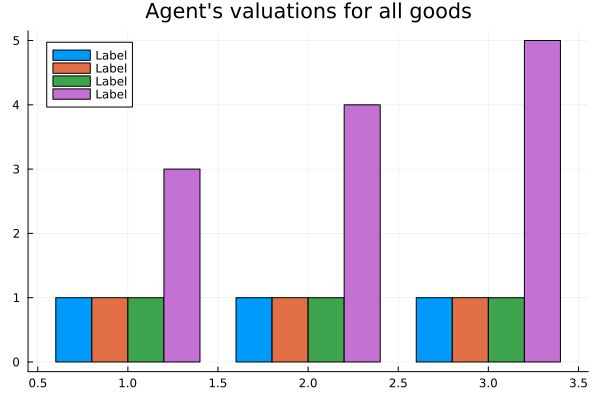
\includegraphics[width=0.8\textwidth]{assets/plots/visualize_instance.png}
    \caption{Visualization of agen's valuations in an instance, these valuations are used in the following figures.}
    \label{fig:visualize_instance}
\end{figure}

\begin{figure}
    \centering
    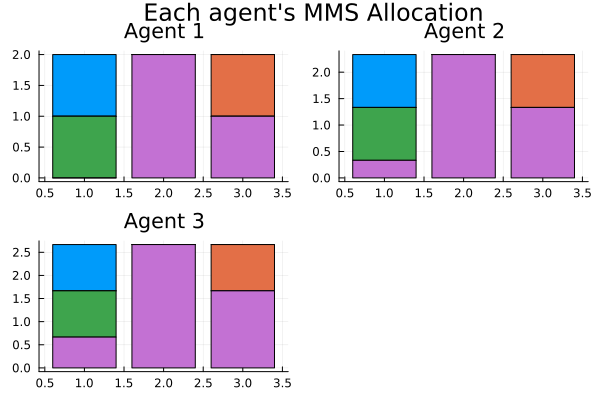
\includegraphics[width=0.8\textwidth]{assets/plots/visualize_mms_allocation.png}
    \caption{Visualization of each agents MMS Allocation for the mixed instance.}
    \label{fig:visualize_mms_allocation}
\end{figure}


\begin{figure}
    \centering
    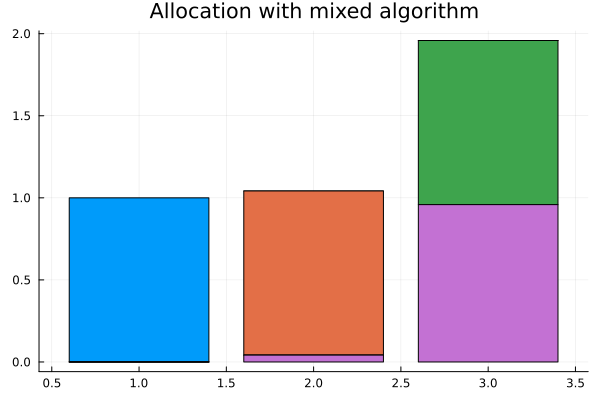
\includegraphics[width=0.8\textwidth]{assets/plots/visualize_mixed_allocation.png}
    \caption{Visualization of each agents MMS Allocation for the mixed instance.}
    \label{fig:visualize_mixed_allocation}
\end{figure}


\begin{figure}
    \centering
    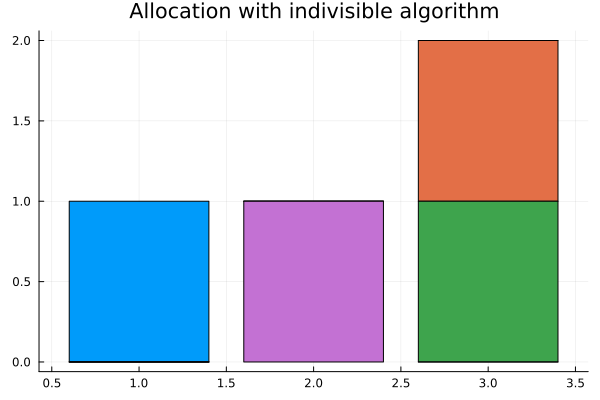
\includegraphics[width=0.8\textwidth]{assets/plots/visualize_indivisible_allocation.png}
    \caption{Visualization of each agents MMS Allocation for the mixed instance.}
    \label{fig:visualize_indivisible_allocation}
\end{figure}

\begin{figure}
    \centering
    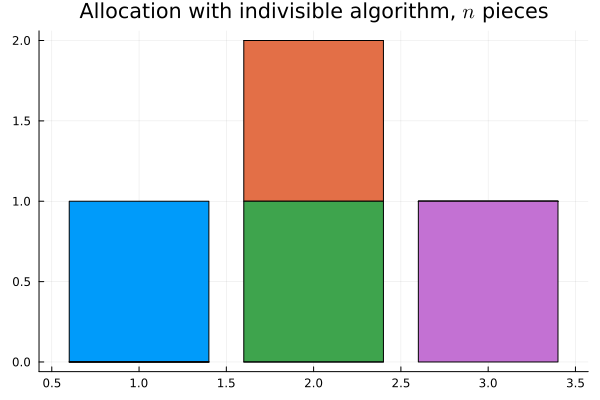
\includegraphics[width=0.8\textwidth]{assets/plots/visualize_indivisible_n_pieces_allocation.png}
    \caption{Visualization of each agents MMS Allocation for the mixed instance.}
    \label{fig:visualize_indivisible_n_pieces_allocation}
\end{figure}